\section{Metrics for evaluating predictions}

The following metrics can be used to analyze the quality of a \textit{classification model}.

\subsection{Confusion Matrix}

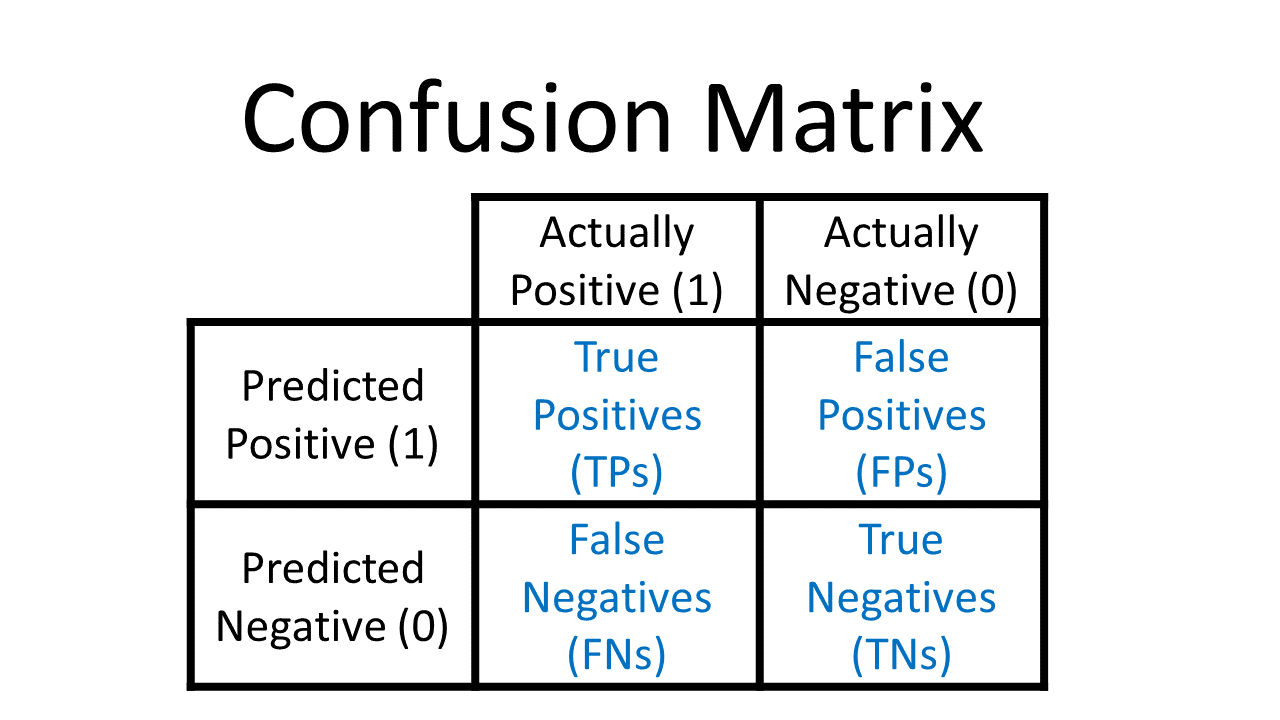
\includegraphics[width=400px]{confusion-matrix.png}

\subsection{Accuracy}

Accuracy answers the question \quotes{\textit{What is the probability that a prediciton is correct?}}.

$$
    Acc = \frac{TP + TN}{TP + TN + FP + FN}
$$

It is only good, if the real distribution of positive and negatives in the data is close to symmetric.

\subsection{Precision}

Precision answers the question \quotes{\textit{If we classify something as positive, how probable is it that it is actually positive?}}.

$$
    Precision = \frac{TP}{TP + FP}
$$

\subsection{Recall}

Recall a.k.a. sensitivity answers the question \quotes{\textit{If a sample is positive, what is the probability we also label it as positive?}}.

$$
    Recall = \frac{TP}{TP + FN}
$$

\subsection{F1 Score}

The F1-score divides the true positives by the sum of the true positives and the mean of the false positives and false negatives. This a high F1-score requires the model to make not few false predictions in either direction. Therefore F1-score is better than accuracy if the real distribution of positive and negative values in the dataset is uneven.

$$
    F1 = 2 \cdot \frac{Precision \cdot Recall}{Precision + Recall} = \frac{TP}{TP + \frac{1}{2} \cdot (FP + FN)}
$$


\section{One-hot encoding}

\section{Overfitting and underfitting}

\subsection{How can it be detected?}

\subsection{Possible solutions}

\section{PCA - principal component analysis}

\subsection{Reasons for using PCA}
\subsection{Selection of good values for compon}

\section{Python Basics}

\subsection{Slicing}
\subsection{Data Extraction with Pandas}

\section{Regularization}
\subsection{What is regularization}
\subsection{Lasso}
\subsection{Ridge}
\subsection{Dropout}

\section{Machine Learning Tasks}

\subsection{Classification}
\subsection{Regression}
\subsection{Clustering}

\section{MLP - Multi-Layer-Perceptron}
\subsection{What is MPL?}
\subsection{Calculation of a number of parameters with and without bias}

\section{Feature map calculation in convolutional NN}

\section{Input and output sizes in Neural networks}
Describe here: Size of inputs and outputs in MLP and convolutional NN calculated from image size and the number of output classes.

\section{Activation functions}
\subsection{Softmax}
\subsection{Sigmoid}
\subsection{RELU}

\section{Solving non-linear problems with NNs}
Use example of logical function XOR here.

\section{K-means}

\section{Gradient Descent}

\section{Hyperparameters of ML models}

\subsection{Learning Rate}
\subsection{Epochs}
\subsection{Regularization}
\subsection{Batch Size}
\subsection{Convolution Kernel size}
\subsection{Max-Pooling}

\section{Logistic Regression and Cross Entropy}


\section{Linear Regression and Normal Equation}


\section{Decision Trees}


\section{K-nearest Neighbors}

